% **************************** %
%          Slides GK           %
% **************************** %

\documentclass[10pt,fleqn]{beamer}
 
% **************************** %
%            Package           %
% **************************** %

% \usepackage{GarmirKhatch}
\usepackage{etex} % pour éviter erreurs de compilation avec tikz
\reserveinserts{20}

\usepackage[utf8]{inputenc}
\usepackage[T1]{fontenc}
\usepackage[french,english]{babel}
\usepackage[french]{layout}
\usepackage{lmodern}
\usepackage{ragged2e}
\usepackage{fancyhdr}
\usepackage{verbatim}
\usepackage{graphicx}
\usepackage{wrapfig}
\usepackage{url}
\usepackage{hyperref}
\usepackage{amsmath}
\usepackage{multirow}
\usepackage{multicol}
\usepackage{array}
\usepackage{colortbl}
\usepackage{comment}
\usepackage{tikz}
\usepackage{tikz-uml}
\usetikzlibrary{positioning, shadows}
\newcommand{\mo}{\textsc{Garmir~Khatch}}

% **************************** %
%          Préambule           %
% **************************** %
% Option pdf
\hypersetup{
      %pdfpagemode = FullScreen,
      pdfauthor   = {AMU FSI 2014},
      pdftitle    = {Présentation du projet TMS pour \mo},
      pdfsubject  = {Système de gestion des transports},
      pdfkeywords = {AMO, GK, TMS, CdC, DAT, PTI}
}
% Thème du pdf 
\usetheme{Warsaw}
% Logo de l'université d'Aix-Marseille
%\logo{\includegraphics[height=6mm]{logo}}
% Affiche les notes
%\setbeameroption{show notes}
% Blocks arrondies et ombrés
\setbeamertemplate{blocks}[rounded][shadow=true] 
% Balle pour la liste d'items
\setbeamertemplate{itemize item}[ball]
% Triangle pour la liste de sous items
\setbeamertemplate{itemize subitem}[triangle]
% Affiche l'ensemble du frame en gris clair
\beamertemplatetransparentcovered
% Faire apparaître un sommaire avant chaque section
\AtBeginSection[]{
	\begin{frame}
		\frametitle{Sommaire}
		\tableofcontents[currentsection, hideallsubsections]
	\end{frame}
}

% **************************** %
%        Page de garde         %
% **************************** %
\title[]{{\Large \textsc{\mo \\ Système de gestion des transports}}}
\author[\textsc{\mo - Système de gestion des transports}]{M2 FSIL - FSI}
\institute{Encadrant : M. Roland \textsc{Agopian}\\
Faculté des Sciences d'Aix-Marseille Université\\
Campus de Luminy}
\date{\scriptsize{ 27 mars 2014}}

% **************************** %
%       Corps du document      %
% **************************** %
\begin{document}
 
% **************************** %
%            Entête            %
% **************************** %
\begin{frame}
\begin{figure}
\centering

\includegraphics[scale=0.52]{Images/EnTeteSciences}
\end{figure}
\titlepage
\end{frame}

\begin{frame}
\frametitle{Sommaire}
\tableofcontents[hideallsubsections]
\end{frame}

\section*{Gantt général}

% Présentation sommaire : AMO -> ME + GANTT de ces 2 taches

\section[Mission d'AMO]{Mission d'AMO}
%Les termes AMO, MO, ME seront utilisés. Est-il nécessaire de les expliciter~?

\subsection{Mission d'AMO~: Jalonnements}
\begin{frame}
	\frametitle{Mission d'AMO~: Jalonnements}
\end{frame}

\begin{frame}
	\centering
	\begin{block}{Gestion de projet}
	\begin{enumerate}
		\item Étude de faisabilité\pause
		\item Expression du besoin\pause
		\item Validation du besoin\pause
		\item Réponse au besoin\pause
		\item Choix de la solution\pause
		\item Conception\pause
		\item Réalisation\pause
		\item Vérification\pause
		\item Livraison\pause
		\item Exploitation\pause
	\end{enumerate}
	\end{block}
\end{frame}
s

\subsection{Objectifs pour nous}

\begin{frame}
	\frametitle{Objectifs pour nous}
	\begin{block}{}
		Rédiger et fournir un cahier des charges de consultation au client
	\end{block}
\end{frame}

%Objectif~: Rédaction d'un cahier des charges de consultation


\subsection{Mission d'AMO~: Organisation}
\begin{frame}
	\frametitle{Mission d'AMO~: Organisation} \pause
	\begin{block}{L'organisation générale} \pause
	\begin{itemize}
	\item L'AMO : 2 groupes de 4 étudiants \pause
	\item La MO : Mr Agopian pour le compte d'une société fictive \mo \pause
	\item Réunion hebdomadaire avec le client
	\end{itemize}
	\end{block}
\end{frame}

% Présentation de l'Organisation générale~: 2 groupes de 4 étudiants en tant qu'AMO, la MO Agopian pour le compte d'une société fictive Gk.
%% Réunion chaque semaine. GANTT
%% Agopian mode client vs mode pédagogique.



\subsection{Mission d'AMO~: Présentation de \mo}
\subsubsection{Présentation de \mo}

\begin{frame}
	\frametitle {Présentation de \mo} 
	\begin{block}{Présentation générale} \pause
	\begin{itemize}
	\item L'une des plus grandes organisations humanitaires au monde \pause
	\item Agit avant, pendant et après les catastrophes et les urgences relatives à la santé \pause
	\item Puise sa force de son réseau de volontaires
	\end{itemize}
	\end{block}
\end{frame}

 %% Présentation de Gk et de son projet.
% Gestion de la planification, du suivi, documentaire.
\begin{frame}
\frametitle {Présentation de \mo} \pause
     \begin{figure}[htbp]
	\centering
	\begin{tikzpicture}
		% définition des styles
		\tikzstyle{metier}=[rectangle,draw,fill=yellow!50,text=black]
		\tikzstyle{support}=[rectangle,draw,fill=blue!50,text=black]
		\tikzstyle{supporte}=[->,>=latex,thick,rounded corners=4pt]
		% les nœuds
		\node[metier] (e) at (-3,-3) {Eau et sanitaire};
		\node[metier] (m) at (0,0.5) {Médecine};
		\node[metier] (d) at (3,-3) {Distribution};
		\node[support] (l) at (-2,-1.5) {Logistique};
		\node[support] (t) at (2,-1.5) {Télécoms};
		% les flèches
		\draw[supporte] (l) to[bend left] (t);
		\draw[supporte] (l) to[bend right] (e);
		\draw[supporte] (l) to[bend left] (m);
		\draw[supporte] (l) to[bend right] (d);
		\draw[supporte] (t) to[bend left] (l);
		\draw[supporte] (t) to[bend left] (e);
		\draw[supporte] (t) to[bend right] (m);
		\draw[supporte] (t) to[bend left] (d);
		% la légende
		\draw[supporte] (4,0) -- (7,0) node[midway,above]{Supporte};
	\end{tikzpicture}
	\caption{Dépendances entre les métiers}
\end{figure}  
\end{frame}

\subsubsection{Présentation du projet}

\begin{frame}
\frametitle {Présentation de \mo} \pause
\begin{block}{Processus de la logistique} \pause
\begin{enumerate}
\item Achat \pause
\item Stockage \pause
\item Transport
\end{enumerate}
\end{block}

\begin{block}{Fonctions clefs de la logistique} \pause
\begin{enumerate}
\item Planification/évaluation \pause
\item Acquisition/achat \pause
\item Gestion des entrepôts \pause
\item Organisations des transports \pause
\item Suivi et compte rendu
\end{enumerate}
\end{block}
\end{frame}

\subsubsection{Objectifs du projet}

\begin{frame}
\frametitle {Présentation de \mo} 
\begin{block}{Objectifs de la mission d'AMO pour \mo}
\begin{itemize}
\item Améliorer la qualité de ses services en se dotant d'une solution de type Transport Management System(TMS) 
\item Espérance de retour sur investissement
\end{itemize}
\end{block}
\end{frame}

 \begin{frame}
 \frametitle {Présentation de \mo} 
 
\begin{figure}[htbp] % Arbre à problèmes
	\centering
	\begin{tikzpicture} [
			node distance = 0.4cm, auto,font=\footnotesize,
			% STYLES
			every node/.style={node distance=1.7cm},
			% The comment style is used to describe the characteristics of each force
			comment/.style={rectangle, inner sep= 3pt, text width=2.8cm, node distance=0.2cm, font=\scriptsize\sffamily},
			% The force style is used to draw the forces' name
			force/.style={rectangle, draw, fill=black!10, inner sep=3pt, text width=2.8cm, text badly centered, minimum height=1cm, font=\bfseries\normalsize\sffamily}
		] 
		% Nodes
		\node [force] (confiance) {Confiance\\{\normalfont\footnotesize Envers \mo}};
		\node [force, above of=confiance] (transparent) {Transparence des informations\\{\normalfont\footnotesize Grâce au suivi détaillé}};
		%% Mj %% Bug avec 'X[cm] of transparent' -> Mise ne commentaire et réécriture sans
		\node [force, right=0.6cm of transparent] (serieux) {Sérieux\\{\normalfont\footnotesize Car on peut justifier à tout moment de l'utilisation des ressources}};
		\node [force, left=0.6cm of transparent] (pro) {Professionnalisme\\{\normalfont\footnotesize Notamment grâce à la planification et à l'utilisation optimale du matériel}};
		\node [force, below of=confiance, left=-0.2cm of confiance] (don) {Dons à l'organisation};
		\node [force, below of=confiance, right=-0.2cm of confiance] (benevolat) {Hausse du bénévolat};
%		\node [force, right] (serieux) {Sérieux\\{\normalfont\footnotesize Car on peut justifier à tout moment de l'utilisation des ressources}};
%		\node [force, left] (pro) {Professionnalisme\\{\normalfont\footnotesize Notamment grâce à la planification et à l'utilisation optimale du matériel}};
%		\node [force, below of=confiance, left] (don) {Dons à l'organisation};
%		\node [force, below of=confiance, right] (benevolat) {Hausse du bénévolat};
		% Draw the links between forces
		\path[->,thick]
			(don) edge (confiance)
			(benevolat) edge (confiance)
			(confiance) edge (transparent)
			(confiance) edge (serieux)
			(confiance) edge (pro);
		\end{tikzpicture} 
	\caption{Arbre à problème : Finalité du projet et retour sur investissement}
\end{figure}
 \end{frame}
 
 \begin{frame}
 \frametitle {Présentation de \mo}
 \begin{block}{Nature des prestations demandées}
 \mo recherche  un prestataire pour la réalisation d'une solution TMS, les prestations attendues ~:
 \begin{enumerate}
 \item la suite logicielle \pause
 \item le matériel \pause
 \item le service support
 \end{enumerate}
 \end{block} \pause
 \begin{block}{Parties concernées}
 \begin{enumerate}
 \item Directement: les logisticiens de \mo
 \item Indirectement: les victimes prises en charge
 \end{enumerate}
 \end{block}
 \end{frame}
 
 \begin{frame}
 \frametitle {Architecture générale de la solution attendue}
 \begin{figure}[htbp]
	  \centering
	  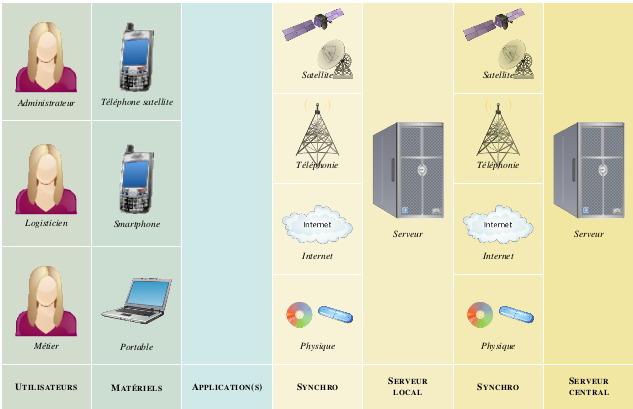
\includegraphics[scale=0.4]{Images/architecture.png}
	  \caption{Architecture generale}
  \end{figure}
 \end{frame}

\subsection{Déroulement de la mission}

\subsubsection{Déroulement de la mission}

\begin{frame}
\frametitle{Déroulement de la mission}
\begin{block}{Déroulement de la mission}
	\begin{enumerate}
	\item Recherche d'une norme
	\item Énoncé du besoin
	\item Expression fonctionnelle du besoin
	\item Cadre de réponse
	\end{enumerate}
	\end{block}
\end{frame}
  
\begin{frame}
	\frametitle{Énoncé du besoin}
	\begin{figure}[htbp]
	\centering
	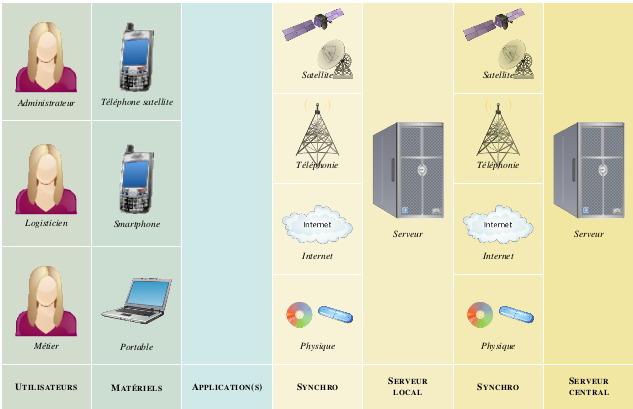
\includegraphics[scale=0.35]{Images/architecture.png}
	\caption{Architecture générale}
	\end{figure}
\end{frame}

\begin{frame}
\frametitle{Expression fonctionnelle du besoin}
\begin{block}{Fonctions de service et de contraintes}
\begin{itemize}
\item la localisation
\item l'interface utilisateur
\item les cas d'utilisations
\end{itemize}
\end{block}
\end{frame}

\begin{frame}
\frametitle{Les cas d'utilisations}
\end{frame}
% Jamais produit de cahier des charges. Nous étions initialement partit sur l'idée des spécifications.
%% Par manque d'expérience, des recherches nous ont menés à trouver une norme définissant le squelette d'un cahier des charges fonctionnel.
%% Norme et non loi. Première erreur a été de suivre sa lettre plutôt que son esprit.
%% PAQ pour le groupe 2.


\subsection{Conclusion}
\begin{frame}
	\frametitle{Conclusion}
\end{frame}

% A terme, les cdcf produit sont spécifiques à GK, à son métier et son contexte.
% Conclusion~: Comment cela s'est-il passé pour groupe1 \& 2~?



\section[Mission de ME]{Mission de ME}

\subsection{Mission de ME~: Jalonnements}
\begin{frame}
	\frametitle{Mission de ME~: Jalonnements}
\end{frame}

\begin{frame}
	\centering
	\begin{block}{Gestion de projet}
	\begin{enumerate}
		\item Étude de faisabilité\pause
		\item Expression du besoin\pause
		\item Validation du besoin\pause
		\item Réponse au besoin\pause
		\item Choix de la solution\pause
		\item Conception\pause
		\item Réalisation\pause
		\item Vérification\pause
		\item Livraison\pause
		\item Exploitation\pause
	\end{enumerate}
	\end{block}
\end{frame}
s

\include{Presentation_Me_Objectif_pour_nous}

\subsection{Organisation}
\begin{frame}
	\frametitle{Organisation}
	\begin{center}
	
\includegraphics[scale=1.2]{Images/organisation}
	\end{center}
\end{frame}


\subsection{Mission de ME~: Authentification et contrôle d'accès}
\begin{frame}
\tableofcontents[subsectionstyle=show/shaded/hide, subsubsectionstyle=hide, sectionstyle=show/hide]
\end{frame}
\begin{frame}
  \frametitle{Authentification et contrôle d'accès}
  \begin{block}{\textbf{ Sommaire }}
  \begin{itemize}
  \item Les choix
  \item Architecture
  \item Gestion des droits
  \item Les Protocoles
  \item Réalisation
  \end{itemize}
  \end{block}
\end{frame}

\begin{frame}
  \frametitle{Authentification et contrôle d'accès : Les choix}
  \begin{block}{\textbf{Pourquoi un annuaire ? }}
  \begin{itemize}
  \item Plus consulté que mis à jour
  \item Structure hierachique 
  \end{itemize} 
  \end{block}
  
  \begin{block}{\textbf{Pourquoi LDAP ? }}
  \begin{itemize}
  \item Protocole réseau léger -> \textbf{Optimisation des flux
}
  \item Authentification et contrôle d'accès -> \textbf{Sécurité}
  \item Haute disponibilité via réplication  -> \textbf{Sécurité}
  \item Mécanisme de référencement
  \end{itemize}
  \end{block}
\end{frame}

  \frametitle{Authentification et contrôle d'accès}
  \begin{figure}[htbp]
	  \centering
	  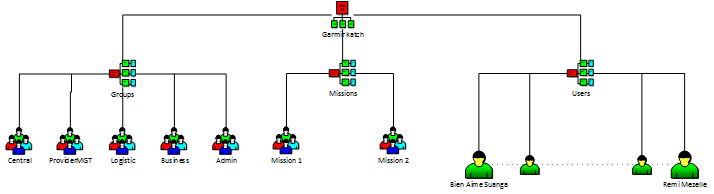
\includegraphics[scale=0.45]{Images/SchemaLDAP.png}
	  \caption{Structure de l'annuaire}
	  \label{SchemaLDAP}
  \end{figure}
 
  \begin{figure}[htbp]
	\centering
	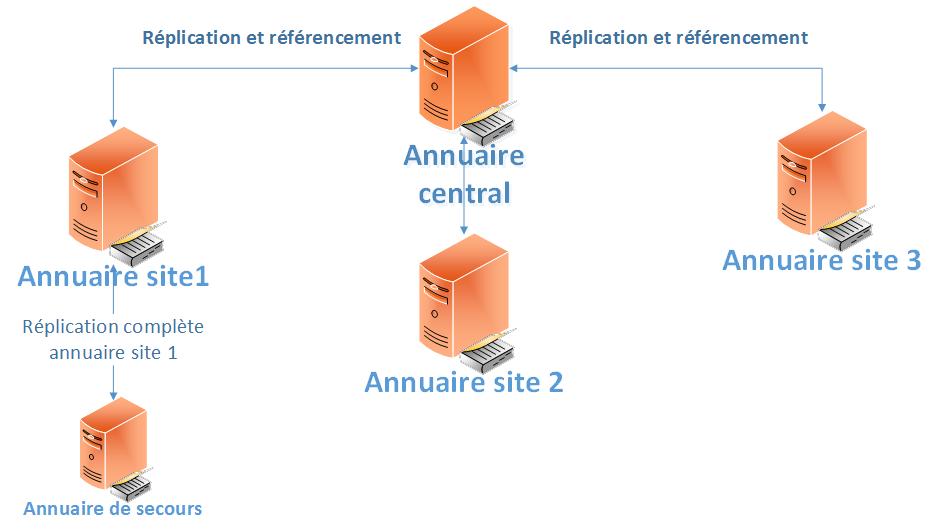
\includegraphics[scale=0.4]{Images/SchemaGlobal.png}
	\caption{Architecture globale}
	\label{SchemaGlobal}
\end{figure}

\begin{figure}[htbp]
	\centering
	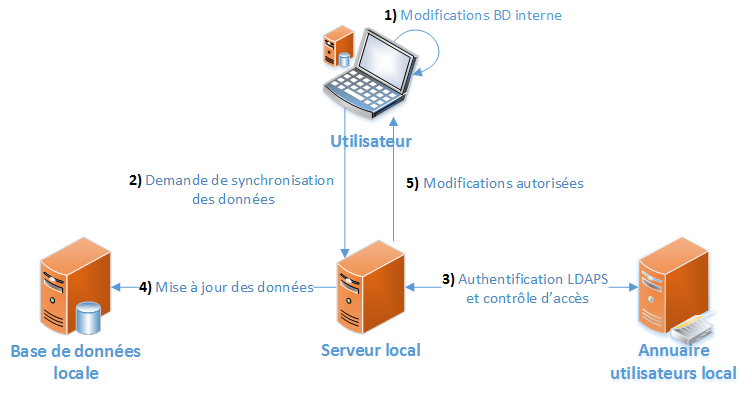
\includegraphics[scale=0.55]{Images/SchemaAuthentification.png}
	\caption{Authentification pour la synchronisation}
	\label{SchemaAuthentification}
\end{figure}

\begin{frame}
  \frametitle{Authentification et contrôle d'accès}
  \begin{block}{\textbf{Droits utilisateurs}}
  \begin{itemize}
  \item Droits pour chaque utilisateur
  \item Droits pour chaque groupe
  \item Autorisations et/ou refus
  \end{itemize}
  \end{block}
\end{frame}

\begin{frame}
  \frametitle{Authentification et contrôle d'accès}
  \begin{block}{\textbf{Gestion des droits}}
  \begin{itemize}
  \item Priorité aux droits directement liés à l'utilisateur 
  \item Priorité aux droits autorisés si l'utilisateur est lié à plusieurs groupes
  \item Les droits du groupe
  \end{itemize}
  \end{block}
\end{frame}

\begin{frame}
  \frametitle{Authentification et contrôle d'accès}
  \begin{block}{\textbf{Autres Protocoles connus}}
  \begin{itemize}
  \item RADIUS (Remote Authentication Dial-In User Service)
  \item PAP (Password Authentication Protocol)
  \item MS-CHAP (Microsoft Challenge Handshake Authentication Protocol)
  \item ... 
  \end{itemize}
  \end{block}
%   Utiles si on sait comment se defendre face à une question
%   \begin{block}{\textbf{Quelques normes utiles}}
%   \begin{itemize}
%   \item X500 
%   \item UDDI : Universal Description Discovery and Integration
%   \item TULLEB : Titre Uniforme Labellisé Librement et Édité(Norme destinée aux annuaires publicitaires)
%   \item ... 
%   \end{itemize}
%   \end{block}
\end{frame}

\begin{frame}
  \frametitle{Authentification et contrôle d'accès}
  \begin{block}{\textbf{Travail effectué}}
  \begin{itemize}
  \item Mise en place du serveur 
    \begin{itemize}
    \item Windows
    \item Linux
    \end{itemize}
  \item Ajout d'un schèma 
  \item Librairie de consulation via l'outil % à rénomer 
  \end{itemize}
  \end{block}

\pause  \begin{block}{\textbf{Ce qui reste à faire}}
  \begin{itemize}
  \item Système de réplication et de référencement 
  \item Ajout et modification dans l'outil
  \end{itemize}
  \end{block}
\end{frame}

\begin{frame}
  \frametitle{Authentification et contrôle d'accès}
  \begin{block}{\textbf{Problèmes rencontrés }}
  \begin{itemize}
  \item Peu de connaissance de l'architecture LDAP
  \item Recherche des librairies LDAP pour Windows 
  
  \end{itemize}
  \end{block}
\end{frame}

% ------------------------------------------------------------------------------
\subsection{Synchronisation}

% ▿▿▿▿▿▿▿▿▿▿▿▿▿▿▿▿▿▿▿▿▿▿▿▿▿▿▿▿▿▿▿▿▿▿▿▿▿▿▿▿▿▿▿▿▿▿▿▿▿▿▿▿▿▿▿▿▿▿▿▿▿▿▿▿▿▿▿▿▿▿▿▿▿▿▿▿▿▿
\begin{frame}
\tableofcontents[subsectionstyle=show/shaded/hide, subsubsectionstyle=hide, sectionstyle=show/hide]
\end{frame}
% ▵▵▵▵▵▵▵▵▵▵▵▵▵▵▵▵▵▵▵▵▵▵▵▵▵▵▵▵▵▵▵▵▵▵▵▵▵▵▵▵▵▵▵▵▵▵▵▵▵▵▵▵▵▵▵▵▵▵▵▵▵▵▵▵▵▵▵▵▵▵▵▵▵▵▵▵▵▵

% ▿▿▿▿▿▿▿▿▿▿▿▿▿▿▿▿▿▿▿▿▿▿▿▿▿▿▿▿▿▿▿▿▿▿▿▿▿▿▿▿▿▿▿▿▿▿▿▿▿▿▿▿▿▿▿▿▿▿▿▿▿▿▿▿▿▿▿▿▿▿▿▿▿▿▿▿▿▿
\begin{frame}
\frametitle{Introduction}

\begin{block}{Contexte}
\begin{itemize}
    \item Liaison réseau pas toujours accessible % Ouragan, tremblements de terre
    \item Plusieurs utilisateurs peuvent modifier la même donnée % Dans le cas où ils sont offline, ça va poser pb
\end{itemize}
\end{block}

\pause

\begin{alertblock}{Problématique}
\begin{itemize}
    \item Cohérence des données
    \item Conflits
\end{itemize}
\end{alertblock}

\end{frame}
% ▵▵▵▵▵▵▵▵▵▵▵▵▵▵▵▵▵▵▵▵▵▵▵▵▵▵▵▵▵▵▵▵▵▵▵▵▵▵▵▵▵▵▵▵▵▵▵▵▵▵▵▵▵▵▵▵▵▵▵▵▵▵▵▵▵▵▵▵▵▵▵▵▵▵▵▵▵▵

% ▿▿▿▿▿▿▿▿▿▿▿▿▿▿▿▿▿▿▿▿▿▿▿▿▿▿▿▿▿▿▿▿▿▿▿▿▿▿▿▿▿▿▿▿▿▿▿▿▿▿▿▿▿▿▿▿▿▿▿▿▿▿▿▿▿▿▿▿▿▿▿▿▿▿▿▿▿▿
\begin{frame}
\frametitle{Introduction}

\begin{exampleblock}{Idée}
\begin{itemize}
    \item Gérer deux modes~: Connecté (synchrone), Hors-ligne (asynchrone)
    \item Logger tout ajout ou modification (avec horodatage)
    \item S'en servir pour la fusion
\end{itemize}
\end{exampleblock}

\end{frame} % Fin de la frame [Introduction]
% ▵▵▵▵▵▵▵▵▵▵▵▵▵▵▵▵▵▵▵▵▵▵▵▵▵▵▵▵▵▵▵▵▵▵▵▵▵▵▵▵▵▵▵▵▵▵▵▵▵▵▵▵▵▵▵▵▵▵▵▵▵▵▵▵▵▵▵▵▵▵▵▵▵▵▵▵▵▵

% ▿▿▿▿▿▿▿▿▿▿▿▿▿▿▿▿▿▿▿▿▿▿▿▿▿▿▿▿▿▿▿▿▿▿▿▿▿▿▿▿▿▿▿▿▿▿▿▿▿▿▿▿▿▿▿▿▿▿▿▿▿▿▿▿▿▿▿▿▿▿▿▿▿▿▿▿▿▿
\begin{frame}
\frametitle{Modes de connexion}
\begin{figure}[htbp]
    \centering
    \scalebox{0.6}{
	    \begin{tikzpicture}
	        % Styles :
		    \tikzstyle{titre}=[rectangle,draw,fill=white,text=black]
		    \tikzstyle{symbole}=[rectangle,text=black, scale=4]
		    \tikzstyle{serveurloc}=[rectangle,draw,fill=blue!50,text=white, minimum height=2cm]
		    \tikzstyle{serveurcen}=[rectangle,draw,fill=yellow!50,text=black, minimum height=2cm]
	        % #### CADRE ROUGE :
		    % Fond :
		    \draw[fill=red!10] (0,0) rectangle (13, 4);
		    % Titres :
		    \node[titre] at (6.50,4.00) {Mode hors-ligne};
		    % Serveurs :
		    \node[serveurloc] at (6.00,2) {Serveur local};
		    \node[serveurcen] at (11.00,2) {Serveur central};
		    \node[symbole] at (8.50,2) {?};
		    \node[symbole] at (3.00,2) {X};
		    % Traits :
		    \draw[line width=2pt] (2, 2) -- (4, 2);
		    \draw[line width=2pt] (7.5, 2) -- (9.5, 2);
		    % Utilisateurs :
		    \umlactor[x=1.00, y=2.00]{Utilisateur}
		    % #### CADRE VERT :
		    % Fond :
		    \draw[fill=green!10] (0,5) rectangle (13, 9);
		    % Titres :
		    \node[titre] at (6.50,9.00) {Mode connecté};
		    % Serveurs :
		    \node[serveurloc] at (6.00,7) {Serveur local};
		    \node[serveurcen] at (11.00,7) {Serveur central};
		    \node[symbole] at (8.50, 7) {?};
		    % Traits :
		    \draw[line width=2pt] (2, 7) -- (4, 7);
		    \draw[line width=2pt] (7.5, 7) -- (9.5, 7);
		    % Utilisateurs :
		    \umlactor[x=1.00, y=7]{Utilisateur}
	    \end{tikzpicture}
    }
	\caption{Topologie des modes connecté et hors-ligne}
	\label{explicationcodeco}
\end{figure}
\end{frame} % Fin de la frame [Synchronisation]
% ▵▵▵▵▵▵▵▵▵▵▵▵▵▵▵▵▵▵▵▵▵▵▵▵▵▵▵▵▵▵▵▵▵▵▵▵▵▵▵▵▵▵▵▵▵▵▵▵▵▵▵▵▵▵▵▵▵▵▵▵▵▵▵▵▵▵▵▵▵▵▵▵▵▵▵▵▵▵

% ▿▿▿▿▿▿▿▿▿▿▿▿▿▿▿▿▿▿▿▿▿▿▿▿▿▿▿▿▿▿▿▿▿▿▿▿▿▿▿▿▿▿▿▿▿▿▿▿▿▿▿▿▿▿▿▿▿▿▿▿▿▿▿▿▿▿▿▿▿▿▿▿▿▿▿▿▿▿
\begin{frame}
\frametitle{Ajout / Modification de donnée}

En simplifié\footnote{Voir DAT, section \emph{3.5.5 Gestion des conflits}, Figures 3.6 \& 3.7} :

\begin{block}{Mode hors-ligne}
\begin{enumerate}
%\setcounter{enumi}{}
    \item Demande d'ajout/modification de l'utilisateur
\end{enumerate}
\vspace{-1em}
\hspace*{.05\linewidth}\begin{minipage}{.9\linewidth}
\begin{exampleblock}{Mode connecté uniquement}
\begin{enumerate}
    \setcounter{enumi}{1}
    \item Demande de permission au serveur
    \item Envoi de l'ajout/modification
    \item Attente de confirmation
\end{enumerate}
\end{exampleblock}
\end{minipage}
\begin{enumerate}
\setcounter{enumi}{4}
    \item (Ssi première \emph{modification} :) \textbf{log} de la donnée originelle
    \item Application des changements en local
    \item \textbf{Log} des détails du changement
\end{enumerate}
\end{block}


\end{frame} % Fin de la frame [Ajout / Modification en mode connecté]
% ▵▵▵▵▵▵▵▵▵▵▵▵▵▵▵▵▵▵▵▵▵▵▵▵▵▵▵▵▵▵▵▵▵▵▵▵▵▵▵▵▵▵▵▵▵▵▵▵▵▵▵▵▵▵▵▵▵▵▵▵▵▵▵▵▵▵▵▵▵▵▵▵▵▵▵▵▵▵

% ▿▿▿▿▿▿▿▿▿▿▿▿▿▿▿▿▿▿▿▿▿▿▿▿▿▿▿▿▿▿▿▿▿▿▿▿▿▿▿▿▿▿▿▿▿▿▿▿▿▿▿▿▿▿▿▿▿▿▿▿▿▿▿▿▿▿▿▿▿▿▿▿▿▿▿▿▿▿
\begin{frame}
\frametitle{Synchronisation}

\begin{block}{Étapes\footnote{Voir DAT, section \emph{3.5.5 Gestion des conflits}, Figure 3.8}}
\begin{enumerate}
    %\setcounter{enumi}{}
    \item Envoi de la date courrante au serveur % Pour pouvoir calculer les éventuels écarts entre la date client et la date serveur
    \item Récupération des logs ultérieurs à la dernière synchronisation
\end{enumerate}
\vspace{-1em}
\hspace*{.05\linewidth}\begin{minipage}{.9\linewidth}
    \begin{block}{Pour chaque donnée modifiée localement :}
    \begin{enumerate}
    \setcounter{enumi}{2}
        \item Vérification des droits
        \item Si conflit : Choix de l'utilisateur entre la donnée locale et la serveur (en fonction de l'originale)
    \end{enumerate}
    \end{block}
\end{minipage}
\begin{enumerate}
\setcounter{enumi}{4}
    \item Application des changements en local
    \item Génération d'\textbf{un} log global des modifications
    \item Envoi au serveur
    \item Attente de confirmation
    \item MAJ de la date de la dernière synchronisation
\end{enumerate}
\end{block} 

\end{frame} % Fin de la frame [Synchronisation]
% ▵▵▵▵▵▵▵▵▵▵▵▵▵▵▵▵▵▵▵▵▵▵▵▵▵▵▵▵▵▵▵▵▵▵▵▵▵▵▵▵▵▵▵▵▵▵▵▵▵▵▵▵▵▵▵▵▵▵▵▵▵▵▵▵▵▵▵▵▵▵▵▵▵▵▵▵▵▵

% ▿▿▿▿▿▿▿▿▿▿▿▿▿▿▿▿▿▿▿▿▿▿▿▿▿▿▿▿▿▿▿▿▿▿▿▿▿▿▿▿▿▿▿▿▿▿▿▿▿▿▿▿▿▿▿▿▿▿▿▿▿▿▿▿▿▿▿▿▿▿▿▿▿▿▿▿▿▿
\begin{frame}
\frametitle{Trafic réseau}

\begin{block}{Communications restreintes}
    \begin{itemize}
        \item GSM ou Satellitaire
        \item Débits faibles
    \end{itemize}
\end{block}

\begin{exampleblock}{Contre-mesures}
\begin{itemize}
    \item Choix des éléments synchronisables
    \item Log unique pour l'ajout/modification (synchronisation)
\end{itemize}
\end{exampleblock}

\end{frame} % Fin de la frame [Gestion du trafic réseau]
% ▵▵▵▵▵▵▵▵▵▵▵▵▵▵▵▵▵▵▵▵▵▵▵▵▵▵▵▵▵▵▵▵▵▵▵▵▵▵▵▵▵▵▵▵▵▵▵▵▵▵▵▵▵▵▵▵▵▵▵▵▵▵▵▵▵▵▵▵▵▵▵▵▵▵▵▵▵▵

% Fin de la sous-section [Synchronisation]
% ------------------------------------------------------------------------------

% ▿▿▿▿▿▿▿▿▿▿▿▿▿▿▿▿▿▿▿▿▿▿▿▿▿▿▿▿▿▿▿▿▿▿▿▿▿▿▿▿▿▿▿▿▿▿▿▿▿▿▿▿▿▿▿▿▿▿▿▿▿▿▿▿▿▿▿▿▿▿▿▿▿▿▿▿▿▿
% ▵▵▵▵▵▵▵▵▵▵▵▵▵▵▵▵▵▵▵▵▵▵▵▵▵▵▵▵▵▵▵▵▵▵▵▵▵▵▵▵▵▵▵▵▵▵▵▵▵▵▵▵▵▵▵▵▵▵▵▵▵▵▵▵▵▵▵▵▵▵▵▵▵▵▵▵▵▵


\subsection{Mission de ME~: Réponse technique au stockage des données}
\begin{frame}
	\frametitle{Mission de ME~: Réponse technique au stockage des données}
\end{frame}

% Fonctionnalité de données~:
%% Problématique~: Stockage des données.
%% Solutions possibles~: SGBDR, XML...
%% Solution choisie \& raisons~: SGBDR MySQL (rebondissement Postgres)
%%% Implémentation, problèmes rencontrés (Driver QMYSQL, solution de contournement SQLite...), etc.


\subsubsection[Nature des données]{Nature des données}

\begin{frame}
\transdissolve[duration=0.2]<1->
\frametitle{Nature des données}
\begin{columns}[c]
\begin{column}{12cm}
\begin{block}{\textbf{Quelle est la nature des données qui vont être stockées ?}}
\begin{itemize}
\item<2-> \textbf{Réquisitions et Waybills}
\item<3-> \textbf{Personnes}
\item<4-> \textbf{Véhicules}
\item<5-> \textbf{Pays}
\item<6-> ...
\end{itemize}
\end{block}
\visible<7>{
$\Rightarrow$ Les données sont donc \textbf{multiples} et de nature \textbf{diverses}.}
\end{column}
\end{columns}
\end{frame}

\subsubsection[Fonctionnalités de base de données]{Fonctionnalités de base de données}

\begin{frame}
\transdissolve[duration=0.2]<2->
\frametitle{Fonctionnalités de base de données}
\begin{columns}[c]
\begin{column}{12cm}
\begin{block}{\textbf{Quelle sont les fonctionnalités attendues ?}}
La base de données en accord avec les besoins formulés dans le CdC de consultation doit permettre~:
\begin{itemize}
\item<2-> \textbf{Gérer les réquisitions \& waybills/delivery~notes (ajout, modification, supprimer)}
\item<3-> \textbf{Faire un suivi des transporteurs, livraisons et des prestataires de service}
\item<4-> \textbf{Gérer les documents administratifs (permis, assurances, contrats, véhicule...)}
\end{itemize}
\end{block}
\end{column}
\end{columns}
\end{frame}

\subsubsection[Problématique relative aux données]{Problématique relative aux données}

\begin{frame}
\transdissolve[duration=0.2]<2->
\frametitle{Problématique relative aux données}
Cette problématique est divisée selon trois points clés~:
\begin{itemize}
	\item<2-> \textbf{Le stockage}
	\item<3-> \textbf{Le transfert}
	\item<4-> \textbf{L'importation~/~exportation}
\end{itemize}
\end{frame}

\subsubsection[Solutions possibles]{Solutions possibles}

\begin{frame}
\transdissolve[duration=0.2]<2->
\frametitle{Solutions possibles}
\begin{columns}
\begin{column}{5cm}
\begin{itemize}[<+->]
	\item<2-> Oracle Database
	\item<3-> PostgreSQL
	\item<4-> MySQL
	\item<5-> Microsoft SQL Server
	\item<6-> SQLite
\end{itemize}
\end{column}
\begin{column}{7cm}

\begin{figure}
\visible<2->{

\includegraphics[scale=0.038]{Images/Oracle}
}\visible<3->{

\includegraphics[scale=0.18]{Images/PostgreSQL}\\
}\visible<4->{

\includegraphics[scale=0.04]{Images/MySQL}\\
}\visible<5->{

\includegraphics[scale=0.052]{Images/MsSqlServer}
}\visible<6->{

\includegraphics[scale=0.052]{Images/SQLite}
}
\end{figure}
\end{column}
\end{columns}
\end{frame}

\subsubsection[Solution retenue]{Solution retenue}

\begin{frame}
\frametitle{Solution retenue}
\begin{columns}
\begin{column}{5cm}
\begin{itemize}
	\item Oracle Database
	\item PostgreSQL
	\item \textbf{MySQL}
	\item Microsoft SQL Server
	\item SQLite
\end{itemize}
\end{column}
\begin{column}{7cm}
\begin{figure}

\includegraphics[scale=0.038]{Images/Oracle}

\includegraphics[scale=0.18]{Images/PostgreSQL}\\

\includegraphics[scale=0.04]{Images/MySQL}\\

\includegraphics[scale=0.052]{Images/MsSqlServer}

\includegraphics[scale=0.052]{Images/SQLite}
\end{figure}
\end{column}
\end{columns}
\end{frame}

\begin{frame}
\transdissolve[duration=0.2]<2->
\frametitle{Solution retenue}
\begin{block}{\textbf{Pourquoi ce SGBDR ?}}
\begin{itemize}
 \item<2-> \textbf{Interopérabilité maximale avec la solution de l'existant}
 \item<3-> \textbf{Solution ne nécessitant pas de coût lié à la formation}
 \item<4-> Solution pouvant facilement s'interfacer à l'aide d'API diverses
 \item<5-> Traitement rapide des requêtes
\end{itemize}
\end{block}
\end{frame}

\subsubsection[Modélisation Conceptuelle et implémentation]{Modélisation Conceptuelle et implémentation}

\begin{frame}
\frametitle{Modélisation Conceptuelle}
La modélisation conceptuelle des données a été réalisé à l'aide de l'outil \textbf{JMerise}.\\
\begin{center}
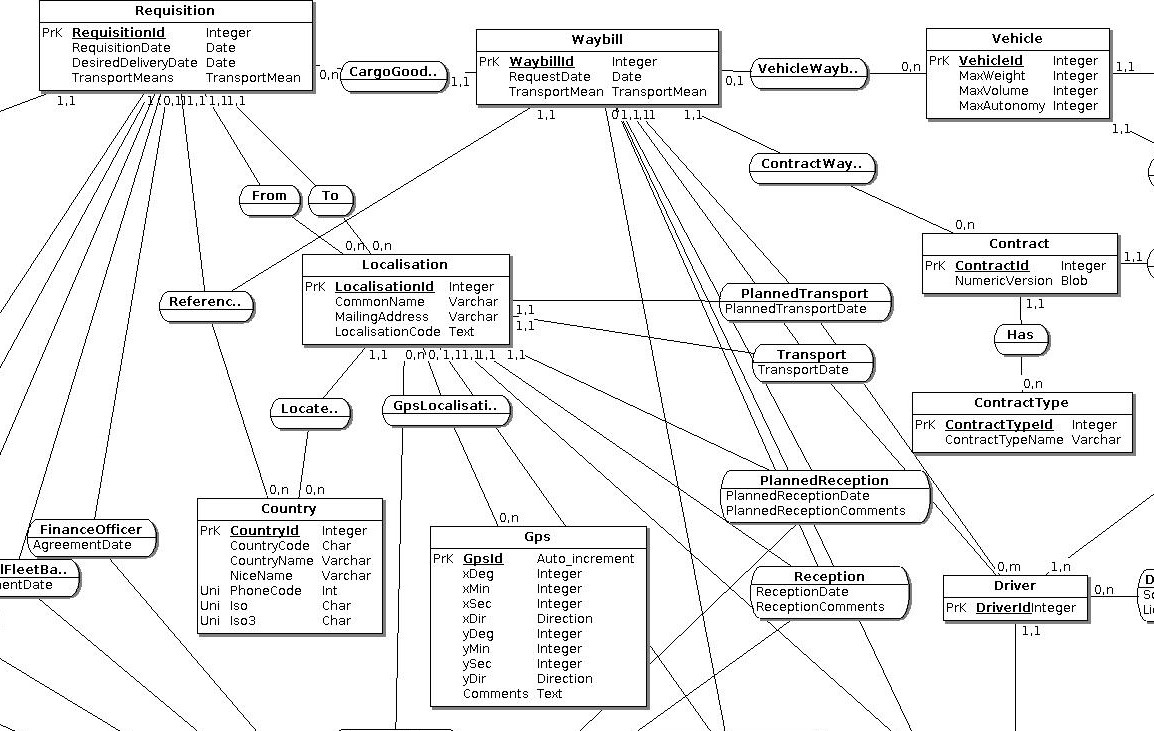
\includegraphics[scale=0.15]{Images/DatabaseSize}
\end{center}
\end{frame}

\begin{frame}
\transdissolve[duration=0.2]<2->
\frametitle{Implémentation}
Le bon fonctionnement de la base de données s'appuie sur les fichiers suivants~:
\begin{enumerate}
	\item<2-> \emph{Database.properties}
	\item<3-> \emph{Database.mcd}
	\item<4-> \emph{Database.sql}
\end{enumerate}
\end{frame}

\subsubsection[Transfert et import~/~export]{Transfert et import~/~export}

\begin{frame}
\frametitle{Transfert et import~/~export}
Le transfert des données se fait par requêtes SQL.\\
Une représentation XML de la base est présente pour limiter le volume de data par compression.\\
\end{frame}

\subsubsection{Difficultés rencontrées}

\begin{frame}
\transdissolve[duration=0.2]<2->
\frametitle{Difficultés rencontrées}
Les principaux problèmes ont été~:
\begin{itemize}
\item<2-> \textbf{Conceptualisation et relations entre les tables}
\item<3-> \textbf{Driver QMYSQL pour Qt et migration}
\end{itemize}
\end{frame}


% Fonctionnalité de sauvegarde~:
%% Problématique~: Sauvegarde, reprise sur pannes...
%% Solutions possibles~:
%% Solution choisie \& raisons~:
%%% Implémentation, problèmes rencontrés (temps...), etc.

\subsection{Mission de ME~: Réponse technique à la sauvegarde et reprise sur panne}
\begin{frame}
\frametitle{Mission de ME~: Réponse technique à la sauvegarde et reprise sur panne}
\begin{block}{\textbf{La sauvegarde : Problématique}}
\begin{itemize}
\item Pas de perte de données
\item Disponibilité
\item Optimisation des flux
\item Coûts
\end{itemize}
\end{block}
\begin{block}{\textbf{Cluster}}
\begin{itemize}
\item groupe logique de serveurs qui s'exécutent simultanément
\item deux postes (configurés comme des serveurs maître/esclave)
\end{itemize}
\end{block}
\end{frame}

\begin{figure}[htbp]
	\centering
	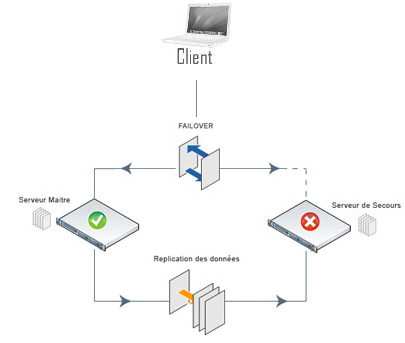
\includegraphics[scale=0.7]{Images/SchemaCluster.png}
	\caption{Cluster, serveur maître et esclave directement connectés}
	\label{SchemaCluster}
\end{figure}

\begin{frame}
\frametitle{}
\begin{block}{\textbf{Fail-Over}}
\begin{itemize}
\item reprise automatique inférieure à une minute
\item mode statique : chaque client est configuré pour basculer sur une URI précise si la standard ne répond plus
\item mode dynamique: le maître fournit dynamiquement l'URI de l'esclave aux clients qui peuvent la mettre à jour
\end{itemize}
\end{block}
\begin{block}{\textbf{Réplication des bases de données en temps réel}}
\begin{itemize}
\item écritures répliquées en temps réel
\item réplication par recopie des journaux de transactions
\item mode synchrone : une transaction émise par un client n'est validée que si l'écriture sur le maître ainsi que la synchronisation avec le serveur de secours sont validées.
\end{itemize}
\end{block}
\end{frame}

\begin{frame}
\begin{block}{\textbf{Procédure de fail-back}}
\begin{itemize}
	\item éteindre le serveur esclave;
	\item copier les données de l'esclave sur le maître;
	\item redémarrer les deux serveurs.
\end{itemize} 
\end{block}
\begin{block}{\textbf{Logiciel}}
\begin{itemize}
	\item Apache Active MQ : agent de messages open source
	\item configurations conservées dans des fichiers XML
\end{itemize} 
\end{block}
\end{frame}


\subsection{Mission de ME~: Cahier de Recette}
\begin{frame}
	\frametitle{Mission de ME~: Cahier de Recette}
\end{frame}

% Cahier de recette (spécifié comme livrable par le CdCF).
%% Problématique~: Tester la solution, ses fonctionnalité, ses performances, son intégration, etc.



\subsection{Mission de ME~: Procédure d'Installation Technique}
\begin{frame}
	\frametitle{Mission de ME~: Procédure d'Installation Technique}
\end{frame}

% Procédure d'installation technique (spécifié comme livrable par le CdCF).



\subsection{Mission de ME~: Conclusion}
\begin{frame}
	\frametitle{Mission de ME~: Conclusion}
\end{frame}

% Listing des éléments de réponse demandés dans le CdCF, et cocher ceux rendus.



\end{document}
